\documentclass[10pt]{beamer}

\usetheme{metropolis}
\definecolor{WiLabRed}{RGB}{197,18,48}
\setbeamercolor{frametitle}{fg=white,bg=WiLabRed}
\setbeamercolor{progress bar}{fg=WiLabRed!90}
\setbeamercolor{title separator}{fg=WiLabRed!90}
\setbeamercolor{progress bar in section page}{fg=WiLabRed!90}
\setbeamercolor{background canvas}{bg=white}
\setbeamercolor{alerted text}{fg=WiLabRed!90}

\usepackage{appendixnumberbeamer}

\usepackage{booktabs}
\usepackage[scale=2]{ccicons}

\usepackage{pgfplots}
\usepgfplotslibrary{dateplot}

\usepackage{xspace}
\newcommand{\themename}{\textbf{\textsc{metropolis}}\xspace}

\usepackage{marvosym}
%\usepackage{subfig}
\usepackage{graphicx}\graphicspath{{images/}}
\usepackage{subcaption}
\usepackage[framed]{./support/mcode}
\usepackage{listings}
\usepackage{amsmath}

\DeclareMathOperator{\sinc}{sinc}
\DeclareMathOperator{\sgn}{sgn}

\title{Laboratory 1 (Part 2): Digital Phase Locked Loops}
\subtitle{\textit{Software Defined Radio for Engineers} (Collins~\textit{et al.}), \textsection{6.3-6.4}}
\date{}
\author{\textbf{Alexander M. Wyglinski, Ph.D.}}
\institute{ \vspace*{1in}\hfill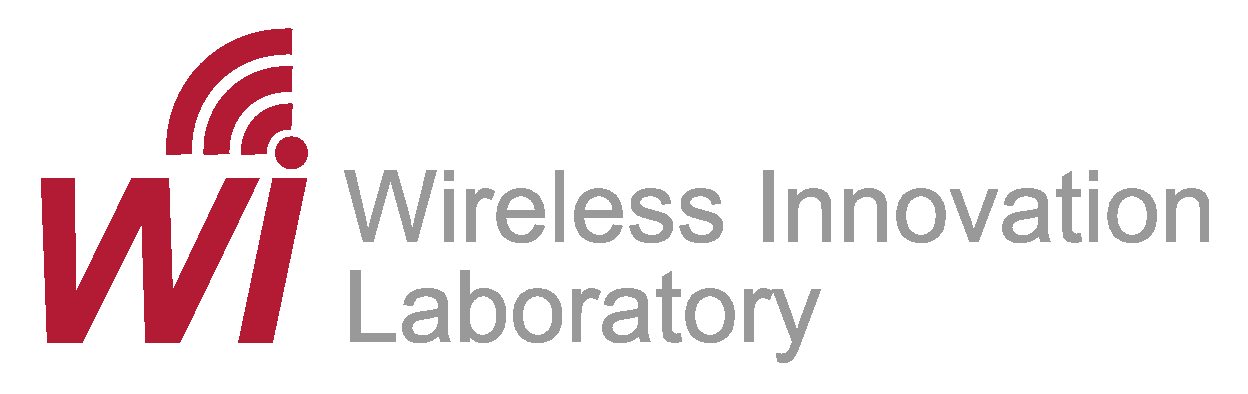
\includegraphics[height=1.125cm]{wilab_logo-A70916.eps} \qquad 
\includegraphics[height=1.125cm]{WPI_Inst_Prim_FulClr.eps}}
% \titlegraphic{\hfill\includegraphics[height=1.5cm]{logo.pdf}}

% Foot for all slides
\setbeamertemplate{frame footer}{\tiny \copyright~2018 by Alexander Wyglinski. This work is licensed under the Creative Commons Attribution-ShareAlike 4.0 International License. To view a copy of this license, visit http://creativecommons.org/licenses/by-sa/4.0/.}

\begin{document}

%\captionsetup[subfigure]{labelformat=empty}

%%%%%%%%%%%%%%%%%%%%%%%%%%%%%%%%%%%%%%%%%%%%%%%%%%%%%%%%%%

\maketitle




%%%%%%%%%%%%%%%%%%%%%%%%%%%%%%%%%%%%%%%%%%%%%%%%%%%%%%%%%%

\begin{frame}[fragile]{Digital Phase Locked Loop Overview}


  \begin{figure}[h]
     \centering
     \includegraphics[width=4in,keepaspectratio=true]{./lab01p02a.eps}
     \caption{Schematic of digital phase locked loop system.}
  \end{figure}

\end{frame}


%%%%%%%%%%%%%%%%%%%%%%%%%%%%%%%%%%%%%%%%%%%%%%%%%%%%%%%%%%

\begin{frame}[fragile]{Digital Phase Locked Loop Functionality}

\begin{itemize}
 \item Ideally when we sample $y(t)$ to get the digital version of it, $y[n]$, we would like to only get the correct samples of the transmission
 \item However, our radios operate on a different clock and there might be a timing offset $\tau$ between transmitter and receiver
 \begin{itemize}
  \item $\tau$ is a fractional timing offset
 \end{itemize} 
 \item We need some sort of way to compensate for $\tau$
 \begin{itemize}
  \item Zero-crossing
  \item M\"{u}ller-Mueller
  \item Gardner
 \end{itemize}
\end{itemize}


\end{frame}

%%%%%%%%%%%%%%%%%%%%%%%%%%%%%%%%%%%%%%%%%%%%%%%%%%%%%%%%%%

\begin{frame}[fragile]{Zero-Crossing Approach}

\begin{itemize}
 \item The goal of the timing error detector (TED) is to obtain an error signal $e[n]$ that is equal to zero
 \begin{itemize}
  \item When this occurs, our interpolator is sampling perfectly at the correct timing instants
 \end{itemize}
 \item The mathematical expression of the TED for determining $e[n]$ is:
 \begin{align}
  e[n]=&\Re\{y((k-0.5)T_s+\tau)\}\cdot\nonumber\\
  &(\sgn(\Re\{y((k-1)T_s+\tau)\})-\sgn(\Re\{y(kT_s+\tau)\}))+\nonumber\\
  &\Im\{y((k-0.5)T_s+\tau)\}\cdot\nonumber\\
  &(\sgn(\Im\{y((k-1)T_s+\tau)\})-\sgn(\Im\{y(kT_s+\tau)\}))
 \end{align}

\end{itemize}


\end{frame}

%%%%%%%%%%%%%%%%%%%%%%%%%%%%%%%%%%%%%%%%%%%%%%%%%%%%%%%%%%

\begin{frame}[fragile]{Timing Error Detection}

So how does this work? 
\begin{itemize}
 \item Suppose our controller chooses a value of $\tau$
 \item If the value of $\tau$ is such that we select the correct sampling instants of two consecutive symbols, then we have one of two possible conditions:
 \begin{itemize}
  \item If both symbols have the same amplitude, then $\sgn(\Re\{y((k-1)T_s+\tau)\})$ and $\sgn(\Re\{y(kT_s+\tau)\})$ should cancel each other out and the $e[n]$ expression should equal zero
  \item If the symbols are of opposite amplitude, then the midway point between them should equal zero and the $e[n]$ expression should equal zero
 \end{itemize}
 \item If the value of $\tau$ is such that we did not select the correct sampling instants of two consecutive symbols, then $e[n]$ will not be equal to zero and we will need to try a new $\tau$
\end{itemize}



\end{frame}


%%%%%%%%%%%%%%%%%%%%%%%%%%%%%%%%%%%%%%%%%%%%%%%%%%%%%%%%%%

\begin{frame}[fragile]{Case 1: Successive Symbols Are Same}


  \begin{figure}[h]
     \centering
     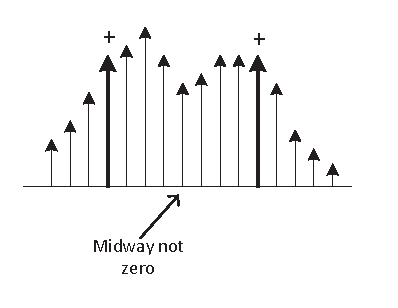
\includegraphics[width=3in,keepaspectratio=true]{./lab01p02b.eps}
     \caption{Schematic of digital phase locked loop system.}
  \end{figure}

\end{frame}


%%%%%%%%%%%%%%%%%%%%%%%%%%%%%%%%%%%%%%%%%%%%%%%%%%%%%%%%%%

\begin{frame}[fragile]{Case 2: Successive Symbols Are Opposite}


  \begin{figure}[h]
     \centering
     \includegraphics[width=3in,keepaspectratio=true]{./lab01p02c.eps}
     \caption{Schematic of digital phase locked loop system.}
  \end{figure}

\end{frame}


%%%%%%%%%%%%%%%%%%%%%%%%%%%%%%%%%%%%%%%%%%%%%%%%%%%%%%%%%%

\begin{frame}[fragile]{Loop Filter Design}

Once we have $e[n]$, the next step is to apply the loop filter
\begin{itemize}
 \item This provides gradual transitions that the controller can act upon such that we avoid rapid variations in the error signal
\end{itemize}

The loop filter is equal to:
\begin{equation}
 F(z)=G_1+\frac{G_2}{1-z^{-1}}
\end{equation}
where:
\begin{align}
 \theta=\frac{B_{\mathrm{Loop}}}{M(\psi+0.25/\psi)},\quad\Delta=1+2\psi\theta+\psi^2\\
 G_1=\frac{4\psi\theta/\Delta}{M},\quad{G_2}=\frac{4|theta^2/\Delta}{M}
\end{align}
such that $B_{\mathrm{Loop}}$ is the loop filter bandwidth and $\psi$ is the preferred dampening factor

\end{frame}


%%%%%%%%%%%%%%%%%%%%%%%%%%%%%%%%%%%%%%%%%%%%%%%%%%%%%%%%%%

\begin{frame}[fragile]{Controller}

The controller is responsible for handling the adjustment of the fractional delay $\tau$ and its application to the interpolator

\end{frame}
%%%%%%%%%%%%%%%%%%%%%%%%%%%%%%%%%%%%%%%%%%%%%%%%%%%%%%%%%%



\end{document}
